\ifdefined\XeTeXrevision\else\pdfoutput=1\fi
% Certified event-proportional video compute: paper draft.
% Build:  tectonic -X compile main.tex   (or: tectonic main.tex)
% For a NeurIPS submission replace the preamble block marked "layout" with \usepackage{neurips_2027}.
\documentclass[10pt]{article}

% ---- layout (stands in for the NeurIPS style file) -------------------------------------------
\usepackage[letterpaper,textwidth=5.5in,textheight=9in,top=1in]{geometry}
\usepackage{times}
\usepackage[T1]{fontenc}
\usepackage[utf8]{inputenc}
\usepackage{microtype}
\setlength{\parskip}{0pt}
\usepackage{titlesec}
\titleformat{\section}{\large\bfseries}{\thesection}{0.8em}{}
\titleformat{\subsection}{\normalsize\bfseries}{\thesubsection}{0.8em}{}
\titleformat{\paragraph}[runin]{\bfseries}{}{0em}{}
\titlespacing{\paragraph}{0pt}{6pt}{4pt}
% ---------------------------------------------------------------------------------------------

\usepackage{amsmath,amssymb,amsthm}
\usepackage{booktabs}
\usepackage{graphicx}
\usepackage{xcolor}
\usepackage{enumitem}
\setlist{nosep,leftmargin=1.4em}
\usepackage[numbers,sort&compress]{natbib}
\usepackage[colorlinks,linkcolor=blue!60!black,citecolor=blue!60!black,urlcolor=blue!60!black]{hyperref}
\usepackage{caption}
\captionsetup{font=small,labelfont=bf}

\theoremstyle{plain}
\newtheorem{theorem}{Theorem}
\newtheorem{proposition}[theorem]{Proposition}
\newtheorem{corollary}[theorem]{Corollary}
\newtheorem{lemma}[theorem]{Lemma}
\theoremstyle{definition}
\newtheorem{definition}[theorem]{Definition}
\theoremstyle{remark}
\newtheorem{remark}[theorem]{Remark}

\newcommand{\Dgm}{\operatorname{Dgm}}
\newcommand{\dB}{d_B}
\newcommand{\range}{\operatorname{range}}
\newcommand{\midrange}{\operatorname{midrange}}
\newcommand{\OPT}{\mathrm{OPT}}
\newcommand{\todo}[1]{\textcolor{red!70!black}{[#1]}}

\title{Certified Event-Proportional Video Compute:\\ Skip Certificates for Moving Cameras, a Bound on What Any Sound Rule Must Keep,\\ and an Audit of Video Token Reducers}

\author{Niyath Nair\\ \texttt{iamniyathnair@gmail.com}}
\date{November 2026}

\begin{document}
\maketitle

\begin{abstract}
Video models spend most of their compute on patches that have not changed, and the rules used to skip them are heuristics that compare a patch with the previous frame and promise nothing about what was discarded. Certified skip replaced the heuristic on fixed cameras by a rule with a theorem: while a patch is skipped, no object of contrast $\Delta$ can have appeared, vanished, split or merged inside it. This paper carries that programme three steps further. (1)~The certificate is extended from sub-pixel translations to a group of warps: a per-frame homography for the camera plus per-patch refinement, with the reference held in a world canvas. The theorem is exact relative to the constructed reference; the one approximation, bilinear resampling, enters through an observable per-pixel term $\iota$ that is zero on a fixed camera and is reported wherever it is not. On the 90 moving-camera clips of DAVIS~2017 the rule drops a median of 72.8\% of patches where the best fixed-camera rule drops 43.5\%, almost all of it on the background, with zero violations in 20{,}242 audited patches; on three excerpts of a film with cuts it drops 71.5\% against 61.5\%. (2)~We ask how many patches any rule with the same guarantee must keep. For any seminorm statistic, the causal anchored rule at threshold $\Delta$ keeps at most twice as many patches as a clairvoyant schedule at threshold $\Delta/2$, plus one, and no deterministic causal rule can be competitive at any guarantee tighter than $\Delta/2$; on footage the rule is within 1--18\% of the clairvoyant optimum at the same threshold. (3)~We audit the temporal decision rules of seven published token reducers on planted events at matched budgets. Rules that compare consecutive frames (EVS, run-length tokenization, DyCoke, FrameFusion) miss slow fades unless the frame rate is low relative to the change, as a one-line proposition predicts; rules with periodic, segment or frame-level anchors (PruneVid, LongVU, uniform sampling, periodic refresh) see fades more often but miss brief and small events; the anchored certified rule catches both at the same budget. We also measure what it costs a cached token to refuse the brightness shift the certificate allows: under one point of drop rate at a cap of 16 grey levels. Everything here is at the level of pixels and decision rules; token reuse inside a model and long-video benchmarks are not done and are stated as such.
\end{abstract}

\section{Introduction}

A vision transformer turns every $16 \times 16$ patch of every frame into a token. On a fixed camera almost every patch shows the same wall and floor as a second ago; on a moving camera it shows the same wall, moved. Video language models therefore try to skip tokens, and the systems that do so judge a token redundant by comparing it with the previous frame, with a threshold on a mean difference or a cosine similarity, and say nothing about what was thrown away \citep{choudhury2024rlt,tao2025dycoke,huang2025prunevid,fu2024framefusion,shen2024longvu,yao2025timechatonline}.

\citet{nair2026certifiedskip} asked a different question: can a skip rule come with a theorem naming what cannot have happened in a patch the model did not look at? The answer, for fixed cameras, was a rule that compares each patch with the \emph{last copy sent} and skips while the spread of the change is below a contrast $\Delta$. By stability of persistence diagrams \citep{cohensteiner2007}, no object of contrast $\Delta$ can appear or vanish in a skipped patch, and the threshold cannot be raised. Three further certificates (multi-scale box averages, a quotient by sub-pixel motion, a sequential test for faint persistent change) made the rule usable on real cameras, where it drops a median of 98.9\% of patches across 25 clips. Its stated gaps were moving cameras, token reuse inside a model, the brightness shift that a cached token cannot apply, and the absence of any statement about how much \emph{any} rule with the guarantee must keep.

This paper closes the first and last of those gaps, measures the third, audits the field on the failure mode the certificate was built to avoid, and leaves the second open and says so.

\paragraph{Contributions.}
\begin{enumerate}
\item \textbf{A certificate for moving cameras} (Section~\ref{sec:theory}). The quotient certificate is stated for an arbitrary warp group with the reference held in a world canvas, which makes a per-frame homography plus per-patch refinement a special case. Theorem~\ref{thm:warp} is exact relative to the constructed reference. Proposition~\ref{prop:iota} isolates the only approximation, bilinear resampling, in an observable per-pixel term $\iota$ that the rule reports and that vanishes on a fixed camera, where the construction is the original rule bit for bit. A tightness construction (Proposition~\ref{prop:tight}) survives. On DAVIS~2017 and on a film with cuts the rule is measured against the fixed-camera rules, with object masks separating what it drops on the background from what it keeps on the moving objects.
\item \textbf{A bound on what any sound rule must keep} (Theorem~\ref{thm:opt}). For any seminorm statistic, the anchored rule keeps at most $2\,\OPT_{\Delta/2} + 1$ patches, where $\OPT_\theta$ is the clairvoyant optimum at guarantee $\theta$, and no deterministic causal rule is competitive at any guarantee tighter than $\Delta/2$: the factor two is the exact price of causality. On footage the rule is within 1--18\% of the clairvoyant optimum at the \emph{same} threshold.
\item \textbf{An audit of published token reducers} (Section~\ref{sec:audit}). The temporal decision rules of seven methods are re-implemented at the pixel level and run on planted events at matched budgets. Proposition~\ref{prop:consecutive} says, and the audit confirms, that rules comparing consecutive frames miss change that is slow relative to the frame rate; the audit also finds that rules with periodic anchors see slow change and miss brief and small events. The anchored certified rule sees both at the same budget.
\item \textbf{The shift a cached token cannot carry} (Section~\ref{sec:shift}). The certificate allows a brightness shift $c$; a token reused after the encoder cannot apply it. We give the exact additive correction at a linear embedding and measure the cost of the alternative, a keep rule on $|c|$: under one point of drop rate at a cap of 16 grey levels on three cameras.
\end{enumerate}

\paragraph{What is not in this paper.} No token is reused inside a model; the end-to-end evidence remains the rebuilt-image protocol of \citet{nair2026certifiedskip}. No result on Video-MME, LongVideoBench or MLVU. No certificate through a network. Each is discussed in Section~\ref{sec:limits} with what it would take. Every theoretical claim is either proved or audited numerically with exact persistence diagrams, and the code, outputs and planted-event protocol are in the public repository.

\section{Related work}
\label{sec:related}

\paragraph{Video token reduction.} Run-length tokenization \citep{choudhury2024rlt} compares each spatio-temporal patch with the one at the same position in the previous frame by an $L^1$ pixel difference and merges runs of similar patches into one token with a length encoding. Efficient Video Sampling \citep{evs2025} and TimeChat-Online \citep{yao2025timechatonline} threshold a per-patch difference between consecutive frames inside a video LLM. DyCoke \citep{tao2025dycoke} merges tokens at the same position across groups of four sampled frames by cosine similarity of their encoder features, keeping the first frame of each group, and prunes further by attention in the LLM. FrameFusion \citep{fu2024framefusion} merges adjacent-frame tokens by cosine similarity in early LLM layers and prunes by importance after. PruneVid \citep{huang2025prunevid} segments the video into scenes and merges the tokens that are static across a segment, then clusters spatially. LongVU \citep{shen2024longvu} drops frames whose DINOv2 features are similar to the previous frame's and pools the rest spatially. FastV \citep{chen2024fastv}, VisionZip \citep{yang2025visionzip} and SparseVLM \citep{zhang2024sparsevlm} prune by attention within an image and have no temporal criterion. Section~\ref{sec:audit} re-implements the temporal decision rule of each of the first six in pixel space and says exactly what is kept of the published method; the attention-based methods need the model and are out of scope here. Trajectory tokenization \citep{zhang2025trajectory} assigns one token per panoptic sub-object trajectory, which is the entity-token idea without a certificate; the moving-camera certificate of Section~\ref{sec:theory} is what would let such a token stay frozen with a proof.

\paragraph{Conditional replenishment and deadband sampling.} Sending a sample only when it has drifted by more than a threshold from the last sample sent is conditional replenishment \citep{mounts1969} in video coding and send-on-delta sampling \citep{miskowicz2006} in event-based control. The anchored rule is this idea with a sup-norm statistic; motion-compensated prediction with a residual test is every codec since H.261. What is new in \citet{nair2026certifiedskip} and here is the certificate, the quotient by a motion group, and the competitive analysis of Section~\ref{sec:opt}, which to our knowledge has not been stated for deadband schemes.

\paragraph{Competitive analysis.} Theorem~\ref{thm:opt} is an online-algorithms statement in the sense of \citet{borodin1998}: a causal rule against a clairvoyant optimum, with the resource being keeps and the constraint being soundness. The factor two with a halved guarantee is the usual shape of such results; the proof here is a few lines because the only structure used is the triangle inequality.

\paragraph{Persistence stability and registration.} The certificate rests on the stability theorem for persistence diagrams \citep{cohensteiner2007}. Registration is Lucas--Kanade \citep{lucas1981,baker2004lk} with a Huber loss, a heuristic that affects only how much is kept, never what is certified. Lipschitz constants of attention \citep{kim2021lipschitz} are what a certificate through a network would need; Section~\ref{sec:shift} says why none is claimed.

\section{Background: certified skip on a fixed camera}
\label{sec:background}

A patch $\Omega$ of $P \times P$ pixels ($P = 16$, 8-bit grey) has a reference $R$, the last copy sent to the model, and a new value $F$; $d = F - R$. A \emph{skip rule} is a statistic of $d$ and a threshold; a \emph{certificate} is a theorem of the form ``if the statistic is below the threshold then nothing of the following kind happened in $\Omega$''. Objects are defined by persistent homology: sweeping a level through the sublevel sets of a patch, a dark blob is born at a local minimum and dies when its basin merges into an older one, and its persistence is its contrast; superlevel sets give bright blobs. $\Dgm(g)$ is the multiset of (birth, death) pairs and $\dB$ the bottleneck distance. The one theorem everything rests on is stability \citep{cohensteiner2007}: $\dB(\Dgm g, \Dgm h) \le \lVert g - h \rVert_\infty$.

\paragraph{The range rule.} Skip $\Omega$ iff $s = \max d - \min d < \Delta$; the view of a skipped patch is $R + c$ with $c = \midrange(d)$. Then $\lVert F - (R + c) \rVert_\infty = s/2 < \Delta/2$, hence $\dB(\Dgm F, \Dgm(R + c)) < \Delta/2$: every feature's contrast changes by less than $s$ and no feature of contrast $\ge \Delta$ is born or dies while the patch is skipped. The threshold cannot be raised: for every $d$ with spread $\Delta$ a flat $R$ makes $R + d$ contain a $\Delta$-object. Note the comparison is with the last \emph{kept} copy, never with the previous frame; that choice alone removes the slow-change blind spot of Section~\ref{sec:blind}.

\paragraph{Three refinements.} On real cameras a sub-pixel jitter of a sharp edge changes a one-pixel column by the edge's full contrast, and the range sees it. The \emph{multi-scale} rule replaces the pointwise maximum by the maximum of box averages over boxes of half-width $r$ in a schedule, with thresholds $\Delta_r = \Delta_0 (2r+1)^{-1/2}$; its certificate covers objects that contain a box of each size, at that size's contrast. The \emph{quotient} rule fits a sub-pixel translation per patch and certifies the residual against the translated reference. The \emph{sequential} layer adds a self-normalised space-time scan that catches persistent objects an order of magnitude fainter than any single-frame rule, and only adds keeps, so every skipped patch still carries the memoryless certificate. The recommended operating point, quotient + multi-scale at $\Delta_0 = 80$, drops a median of 99.0\% of patches on 25 fixed-camera clips with 100\% recall of planted small and fading objects; its worst-case certificate is contrast 80 for a single pixel, falling to 30 for an object containing a $7 \times 7$ box. The C++ core runs the full rule at 467~fps at CIF and 89~fps at 720p on one laptop core. All of this, with proofs, measurements and soundness audits, is in \citet{nair2026certifiedskip}; this paper builds on it and does not restate the evidence.

\section{Certificates for moving cameras}
\label{sec:theory}

\subsection{The warp quotient}

Rule~3 of \citet{nair2026certifiedskip} quotients out a sub-pixel translation per patch. Nothing in its proof uses that the warp is a translation; what it uses is that the model holds a token for some reference content and that the rule compares the new patch against a \emph{constructed} image $W$ built from that content. We make the construction explicit for a moving camera and then state what is exact and what is not.

\paragraph{Mechanics.} Kept pixels live in a canvas $C$ in the coordinates of the first frame of the shot. A per-frame map $g_t$ (a homography, estimated by coarse-to-fine Gauss--Newton on brightness constancy with Huber weights so that moving objects do not steer it) sends frame-$t$ pixels to canvas coordinates. For a patch $\Omega$ the rule may further refine $g_t$ by a per-patch translation $\delta$ with $|\delta|_\infty \le \delta_{\max}$, and may choose among several candidate warps (the current registration, the previous one, the nearest whole-pixel translation); write $g$ for the warp finally used on $\Omega$. The warped reference is the bilinear resampling
\begin{equation}
W(x) \;=\; \sum_{k=1}^{4} \lambda_k(x)\, C\big(p_k(x)\big), \qquad p_k(x) \text{ the four canvas pixels around } g(x),\ \lambda_k \ge 0,\ \textstyle\sum_k \lambda_k = 1 .
\label{eq:W}
\end{equation}
With $d = F - W$ on $\Omega$, $s = \range(d) = \max d - \min d$ and $c = \midrange(d)$, the patch is dropped iff $s < \Delta$ (range certificate) or iff every box statistic of $d - c$ is below its scale's threshold (multi-scale certificate, \citealp[Rule 2]{nair2026certifiedskip}). A patch whose sampling region is not yet in the canvas has no reference and is kept. Kept patches are written into the canvas by inverse warping, one bilinear resample per canvas pixel. A frame on which the registration fails (robust residual scale above $24$ grey levels) is a shot cut: the canvas is reset to that frame and every patch is kept, so cut-heavy footage pays for its cuts.

\begin{theorem}[warp-quotient certificate]
\label{thm:warp}
Let $g$ be any map $\Omega \to \mathbb{R}^2$ and $W$ any image on $\Omega$ built from previously kept pixels, in particular \eqref{eq:W}. If the patch is dropped by the range rule then
\begin{enumerate}[label=(\alph*)]
\item $\lVert F - (W + c) \rVert_\infty = s/2 < \Delta/2$;
\item $\dB\big(\Dgm F,\ \Dgm(W + c)\big) \le s/2 < \Delta/2$ for sublevel-set and for superlevel-set $H_0$ (dark and bright blobs);
\item every feature's contrast changes by at most $s$, and no feature of contrast $\ge \Delta$ is born from nothing or dies into nothing in $F$ relative to $W$.
\end{enumerate}
If the patch is dropped by the multi-scale rule with thresholds $\varepsilon_r$, then for every box half-width $r$ in the schedule, $\dB\big(\Dgm(\beta_r F), \Dgm(\beta_r(W + c))\big) < \varepsilon_r$ for the $(2r{+}1)$-box mean filter $\beta_r$, and no feature of $\beta_r F$ with persistence $\ge 2\varepsilon_r$ is created or destroyed relative to $\beta_r W$.
\end{theorem}

\begin{proof}
(a) For every pixel $d(x) - c \in [\min d - c, \max d - c] = [-s/2, s/2]$, both ends attained. (b) is the stability theorem of \citet{cohensteiner2007} applied to $F$ and $W + c$; adding the constant $c$ shifts births and deaths of $W$ equally and leaves persistences unchanged. (c) In a bottleneck matching of cost $\le s/2$ a matched feature's birth and death each move by at most $s/2$ and an unmatched feature has persistence at most $s < \Delta$. The multi-scale statement is \citet[Theorem 5]{nair2026certifiedskip} with $R + c$ replaced by $W + c$; its proof uses only linearity of $\beta_r$ and stability.
\end{proof}

The theorem is exact and says nothing about how $g$ was found: registration is a heuristic that affects only how many patches are kept. What it leaves open is how $W$ relates to the pixels that were actually kept, which is where interpolation enters.

\begin{proposition}[where interpolation enters, and by how much]
\label{prop:iota}
Each canvas value in \eqref{eq:W} is itself a convex combination of four pixels of the frame that wrote it, $C(p_k) = \sum_{j=1}^{4} \mu_{kj} F_{t_k}(q_{kj})$. Let $W_{\mathrm{NN}}(x) = F_{t_{k^*}}(q_{k^* j^*})$ be the kept pixel at the nearest read corner $k^*$ and its nearest write corner $j^*$, an actual pixel value of a kept frame, and let
\[
\iota(x) \;=\; \operatorname{osc}_k C(p_k(x)) \;+\; \max_k \operatorname{osc}_j F_{t_k}(q_{kj}),
\qquad \operatorname{osc} = \max - \min .
\]
Then $|W(x) - W_{\mathrm{NN}}(x)| \le \iota(x)$ for every pixel, and with $\iota(\Omega) = \max_{x \in \Omega} \iota(x)$,
\[
\dB\big(\Dgm F,\ \Dgm(W_{\mathrm{NN}} + c)\big) \;<\; \Delta/2 + \iota(\Omega)
\]
on every dropped patch. If $g$ maps $\Omega$ onto whole canvas pixels that were written at whole pixel positions, $\iota \equiv 0$ on $\Omega$.
\end{proposition}

\begin{proof}
$W(x)$ lies in the convex hull of the four corner values, so $|W(x) - C(p_{k^*})| \le \operatorname{osc}_k C(p_k)$; likewise $|C(p_{k^*}) - F_{t_{k^*}}(q_{k^* j^*})| \le \operatorname{osc}_j F_{t_{k^*}}(q_{k^* j}) \le \max_k \operatorname{osc}_j F_{t_k}(q_{kj})$. Add. The diagram statement is Theorem~\ref{thm:warp}(b), the triangle inequality for $\dB$ and stability applied to $W$ and $W_{\mathrm{NN}}$. For whole-pixel positions all four weights but one vanish at both stages and the oscillations are of a single value.
\end{proof}

$\iota$ is observable: the rule computes it per pixel and reports it per patch and per frame. It is zero on every patch of a fixed camera, where the construction reduces bit for bit to the range rule (Appendix~\ref{app:parity}), and it is large exactly where the reference has an edge sharper than one pixel under the sample point, which is the one place where the position of content is ambiguous at the level of the edge's contrast. What Proposition~\ref{prop:iota} does \emph{not} say is that $\Dgm(W_{\mathrm{NN}})$ is the diagram of the kept content ``moved by $g$'': for a whole-pixel translation that is literally true, since $W_{\mathrm{NN}}$ restricted to $\Omega$ is a block of kept pixels; for a general warp the pull-back by the rounded map can change grid adjacency, and we do not have a bound. We measure it instead (Section~\ref{sec:warpaudit}): on synthetic scenes re-rendered under sub-pixel translations and random homographies, $W$ never has fewer features of contrast $\ge \Delta - 2\iota$ than the re-indexed kept pixels have of contrast $\ge \Delta$.

\begin{proposition}[tightness]
\label{prop:tight}
For every warp $g$ and every residual pattern $e$ on $\Omega$ with $\range(e) = \Delta$ there is a canvas, a flat one, on which $F = W + e$ contains a feature of contrast exactly $\Delta$ that $W$ does not. Hence no rule that reads only the residual against some $g$ in the group can drop at residual spread $\ge \Delta$ and keep Theorem~\ref{thm:warp}.
\end{proposition}

\begin{proof}
A warp of a flat canvas is flat, so $W$ has no features and the deepest minimum of $W + e$ is a dark blob of persistence $\Delta$ (\citealp[Proposition 2]{nair2026certifiedskip}).
\end{proof}

\paragraph{What the token means.} The model holds a token for the content of $\Omega$'s reference. Theorem~\ref{thm:warp} says the new frame is that content, moved by $g$ and shifted by $c$, up to $\Delta$-contrast topology; Proposition~\ref{prop:iota} says ``that content'' means the kept pixels up to $\iota$. A background token therefore stays frozen \emph{modulo the frame warp}, which is the design of an entity token: the warp is metadata that travels with the token, not a reason to recompute it. What the token cannot absorb is $c$; Section~\ref{sec:shift} measures what it costs to refuse it.

\subsection{How much must any sound rule keep?}
\label{sec:opt}

Every certificate above is a promise of the same shape: on a skipped patch, the content the model holds is within $\theta$ of the truth in the currency of a statistic $\sigma$. We ask how many patches that promise forces \emph{any} rule to keep, with or without foresight.

\begin{definition}
Fix a patch and a statistic $\sigma$ on patch differences that is a seminorm: $\sigma(a + b) \le \sigma(a) + \sigma(b)$, $\sigma(-a) = \sigma(a)$. The range, the $L^1$ mean, the flat norm and the multi-scale statistic with the brightness shift optimised out are seminorms. A \emph{schedule} is a set of keep times containing $0$; its anchor at time $t$ is the last keep $\le t$. The schedule is \emph{$\theta$-sound} if $\sigma(F_t - F_{a(t)}) < \theta$ at every skipped $t$. The \emph{anchored rule} at threshold $\Delta$ keeps exactly when $\sigma(F_t - F_{a(t)}) \ge \Delta$; write $m_\Delta$ for its number of keeps. $\OPT_\theta$ is the fewest keeps of any $\theta$-sound schedule, chosen with full knowledge of the sequence.
\end{definition}

The range rule, the multi-scale rule (with $c$ optimised) and the anchored mean rule are anchored rules for their statistics; consecutive-frame rules are not schedules of this kind at all, since they promise nothing about the held content.

\begin{theorem}[the price of causality is a factor two in the guarantee]
\label{thm:opt}
For every sequence and every seminorm $\sigma$:
\begin{enumerate}[label=(\roman*)]
\item $\OPT_\Delta \le m_\Delta$;
\item $m_\Delta \le 2\,\OPT_{\Delta/2} + 1$;
\item for every $\gamma < 2$ and every deterministic causal $\Delta$-sound rule $A$ there are sequences on which $A$ keeps every frame while $\OPT_{\Delta/\gamma} \le 2$.
\end{enumerate}
\end{theorem}

\begin{proof}
(i) The anchored rule is $\Delta$-sound by construction.
(ii) Let $g_1 < \dots < g_m$ be the anchored rule's keeps. Suppose a $\Delta/2$-sound schedule $S$ keeps nowhere in the closed interval $[g_i, g_{i+1}]$. Then both endpoints share an anchor $a < g_i$ of $S$, and
$\sigma(F_{g_{i+1}} - F_{g_i}) \le \sigma(F_{g_{i+1}} - F_a) + \sigma(F_a - F_{g_i}) < \Delta/2 + \Delta/2$,
contradicting the rule's keep at $g_{i+1}$ (it kept because $\sigma(F_{g_{i+1}} - F_{g_i}) \ge \Delta$, $g_i$ being its anchor). So $S$ keeps in each of the $m - 1$ closed intervals; a keep at a shared endpoint serves two of them, hence $|S| \ge \lceil (m-1)/2 \rceil$.
(iii) Take scalar multiples $x_t$ of one pattern $p$ with $\sigma(p) = 1$, so $\sigma(F_t - F_a) = |x_t - x_a|$, and put $u = (\Delta/\gamma)(1 - \epsilon)$ with $\epsilon$ small. Send $x_0 = 0$, $x_1 = u$. If $A$ keeps at $1$, its anchor is $u$ and the adversary alternates $x_t = \pm u$: consecutive values are $2u \ge \Delta$ apart, so every frame is forced, while the anchor $0$ covers every value since $|u| < \Delta/\gamma$: $\OPT_{\Delta/\gamma} = 1$. If $A$ skips at $1$, send $x_2 = \Delta$, which forces a keep, and then alternate between $-\epsilon'$ and $2u - 2\epsilon'$ with $\epsilon' = \epsilon\Delta/(2\gamma)$. Both values are within $\Delta/\gamma$ of $u$, so the clairvoyant schedule that keeps at $0$ and $1$ is $\Delta/\gamma$-sound and $\OPT_{\Delta/\gamma} = 2$; and each value is at distance $\ge \Delta$ from $A$'s anchor, which is always the previous frame, for $\gamma < 2 - 2.5\epsilon$. Voluntary keeps by $A$ only move its anchor to a value the adversary treats the same way, and $A$ is deterministic, so the adversary can branch on its decision at frame~$1$.
\end{proof}

Three readings. First, $m_\Delta$ can exceed $\OPT_\Delta$ by an unbounded factor (a sequence that alternates around a value the rule never anchors on), so the comparison at equal threshold is the wrong one; (iii) says it is wrong for every causal rule, not just ours. Second, at half the guarantee the anchored rule is within a factor two of clairvoyance, for any seminorm, and nothing causal does better than that factor. Third, the sequences of (iii) are adversarial; on footage, Section~\ref{sec:exp} finds $m_\Delta / \OPT_\Delta$ between $1.00$ and $1.18$, so the causal rule is near-optimal in practice at the \emph{same} guarantee, with the factor two held in reserve for the worst case. Theorem~\ref{thm:opt} applies verbatim to the warp rule of Section~\ref{sec:theory} for a fixed warp; with a warp that changes between frames the triangle inequality picks up the interpolation term, and we do not state a bound.

\subsection{Why consecutive comparison misses slow change}
\label{sec:blind}

Most published reducers judge a token redundant by comparing it with the \emph{previous frame} (Section~\ref{sec:related}). The following is elementary and is the whole mechanism behind the audit of Section~\ref{sec:audit}.

\begin{proposition}[consecutive comparison]
\label{prop:consecutive}
Let a rule skip patch $\Omega$ at time $t$ iff $\sigma(F_t - F_{t-1}) < \tau$ for a seminorm $\sigma$, and let $\Omega$ carry a change with per-frame increments $i_t$ on top of noise $n_t$, $F_t = F_0 + \sum_{k \le t} i_k + n_t$. If $\sigma(i_t) \le \tau - \sigma(n_t - n_{t-1})$ for all $t$ in a window, the patch is skipped throughout the window, whatever $\sum_t i_t$ becomes. In particular a fade whose per-frame increment is below $\tau$ minus the noise spread is never sent, while an anchored rule sends it once $\sigma\big(\sum_{k \le t} i_k + n_t - n_{t_0}\big)$ reaches its threshold.
\end{proposition}

\begin{proof}
$\sigma(F_t - F_{t-1}) \le \sigma(i_t) + \sigma(n_t - n_{t-1}) < \tau$ by the triangle inequality.
\end{proof}

When the noise does exceed $\tau - \sigma(i_t)$ on some frames, the consecutive rule fires on the fading patch at that patch's own static false-fire rate, which does not depend on the fade. A budget that drops a fraction $D$ of patches on static footage bounds the \emph{average} rate by $1 - D$, but the rate on a quiet patch is far below the average, because a calibrated rule spends its budget on the moving regions; Section~\ref{sec:audit} measures both. The same proposition applies to rules that compare within a short segment (the segment's first frame is the anchor, and a fade longer than the segment is a slow change relative to it) and to frame-level similarity rules, where a small region's change is diluted over the frame before it is compared.

\subsection{What a cached token can and cannot carry}
\label{sec:shift}

A dropped patch is certified equal to its reference \emph{up to the brightness shift $c$}. The view adds $c$ back; a token cached inside a model cannot, unless the map from pixels to that token is affine.

\begin{proposition}[the shift through a linear patch embedding]
\label{prop:shift}
Let $E$ be a linear patch embedding, $E(W) = A\,\mathrm{vec}(W) + b$ (a convolution with stride equal to the patch, as in SigLIP- and Qwen2-VL-style encoders). Then $E(W + c\,\mathbf 1) = E(W) + c\,A\mathbf 1$ exactly, where $A\mathbf 1$ is the per-channel sum of the kernel, computed once. No such identity holds after the first nonlinearity.
\end{proposition}

So the shift can be injected exactly at the embedding, which saves only the embedding; a token reused \emph{after} the encoder has no exact correction. The alternative is a keep rule: send the patch whenever $|c|$ exceeds a cap $\kappa$, so that every reused token is within $\Delta/2 + \kappa$ of the truth pointwise with nothing to apply. The rule already supports the cap; Section~\ref{sec:exp} measures its cost in drop rate on three cameras.

\paragraph{Through the network.} For a composition of layers with Lipschitz constants $L_\ell$, an input certificate $\lVert F - (W + c) \rVert \le \varepsilon$ gives $\lVert y_{\mathrm{full}} - y_{\mathrm{skip}} \rVert \le (\prod_\ell L_\ell)\,\varepsilon$. Dot-product attention is not Lipschitz on an unbounded domain \citep{kim2021lipschitz}, so for a standard encoder the product is either undefined or vacuous. We state this as the open problem it is and do not claim a bound through any model in this paper.

\section{An audit of video token reducers}
\label{sec:audit}

Proposition~\ref{prop:consecutive} predicts which reducers miss slow change. Here we test the prediction, and the converse question of what anchored rules miss, on planted events at matched budgets.

\paragraph{What is re-implemented.} No published system is run. Each method is reduced to the temporal comparison that decides whether a token is redundant, with the model-side statistic replaced by the pixel-space statistic that plays the same role (Appendix~\ref{app:reducers}). Seven methods reduce to four comparisons. \emph{Consecutive mean}: mean $|F_t - F_{t-1}|$ per patch below $\tau$, the pixel test of EVS \citep{evs2025} and a per-frame analogue of the normalised-pixel $L^1$ test of run-length tokenization \citep{choudhury2024rlt}; EVS's percentile cutoff is a threshold set by the budget, which is what calibration does. \emph{Consecutive cosine}: cosine similarity of patch vectors of $F_t$ and $F_{t-1}$ above $1 - \tau$, with mean-removed random projections standing in for a linear patch embedding: the feature test of TimeChat-Online \citep{yao2025timechatonline} and FrameFusion \citep{fu2024framefusion}, and the adjacent-frame part of DyCoke \citep{tao2025dycoke}. \emph{Segment static}: within fixed 16-frame segments, a patch position is static iff the mean pairwise cosine similarity of its patch vectors over the segment's frames is at least $1 - \tau$, and a static position is kept once per segment: the static-token test of PruneVid \citep{huang2025prunevid}, with fixed segments in place of its clustering. \emph{Window similarity}: within non-overlapping 8-frame windows, a whole frame is dropped iff its mean cosine similarity to the window's other frames is at least $1 - \tau$: the temporal reduction of LongVU \citep{shen2024longvu}, without its query-guided and spatial steps. Three reference rules complete the set: the consecutive mean with a full refresh every 60 frames, uniform frame sampling, and the anchored mean (mean $|F_t - R|$ against the last kept copy, the anchored rule with no certificate). The certified rules are the range rule, quotient + multi-scale at $\Delta_0 = 80$, and the same with the sequential layer \citep{nair2026certifiedskip}. What this tests is the comparison structure of each method, not its accuracy as a system: a learned feature can be more or less sensitive than a pixel statistic, but it cannot see a change against a frame it is not compared with.

\paragraph{Protocol.} Six kinds of event are planted into real fixed-camera footage (Appendix~\ref{app:events}): a small $5{\times}5$ object of contrast 40 for one frame (30 events); a tiny $3{\times}3$ object of contrast 48 for one frame (30); a fade of an $8{\times}8$ square to contrast 48 over 3~s (20); a slow fade of a $12{\times}12$ square to contrast 48 over 12~s (20); a $6{\times}6$ mover of contrast 40 at 2~px per frame for 12 frames (15); and a faint persistent $6{\times}6$ object of contrast 12 for 3~s (15). A one-frame or moving event is caught if its patch is kept while the object is present; a faint object if it is kept within 1~s; a fade if it is kept at or before the frame where the fade reaches contrast 32. Every rule's threshold is calibrated on the untouched clip to the drop rate of the certified quotient + multi-scale rule at $\Delta_0 = 80$, so all rules spend the same budget: every thresholded rule matches it to within 0.001. Three rules move in whole frames (uniform sampling, LongVU's frame rule, the periodic refresh) and are shown at their nearest setting, within 0.003 except the refresh on VIRAT, whose keyframes alone exceed the budget and which therefore gets 1.7--1.9 times the tokens of the others. Two clips (the CAVIAR lobby \citep{caviar2004} and VIRAT~S\_000200\_00 \citep{oh2011virat}) are run at their native rates (25 and 10~fps) and at 2~fps, the rate at which a video LLM is usually fed. The column $\rho$ is the rule's median false-fire rate on the fading patches before their fade starts.

\begin{table}[t]
\centering\scriptsize
\setlength{\tabcolsep}{3.5pt}
\resizebox{\linewidth}{!}{\begin{tabular}{lrrrrrrrrr}
\toprule
rule & drop & tokens/s & small 5$\times$5 & tiny 3$\times$3 & fade 3 s & fade 12 s & mover & faint 12 & $\rho$ median \\
\midrule
certified range & 0.976 & 263 & 0.07 & 0.13 & 0.15 & 0.25 & 0.08 & 0.13 & 0.000 \\
certified quotient+MS & 0.977 & 246 & 1.00 & 1.00 & 1.00 & 0.95 & 0.90 & 0.20 & 0.000 \\
certified +sequential & 0.977 & 251 & 1.00 & 1.00 & 1.00 & 0.95 & 0.91 & 1.00 & 0.001 \\
anchored mean (no certificate) & 0.977 & 246 & 0.27 & 0.10 & 1.00 & 1.00 & 0.41 & 0.13 & 0.000 \\
consecutive mean (EVS, RLT) & 0.977 & 246 & 0.10 & 0.03 & 0.05 & 0.15 & 0.16 & 0.07 & 0.000 \\
consecutive cosine (TimeChat, FrameFusion) & 0.977 & 246 & 0.53 & 0.40 & 0.20 & 0.25 & 0.42 & 0.13 & 0.000 \\
segment static (PruneVid) & \multicolumn{9}{l}{cannot reach the budget at this frame rate} \\
window similarity (LongVU) & 0.977 & 249 & 0.03 & 0.03 & 0.00 & 0.15 & 0.05 & 0.07 & 0.031 \\
consecutive + refresh every 60 & 0.977 & 246 & 0.07 & 0.03 & 0.75 & 1.00 & 0.04 & 0.33 & 0.016 \\
uniform frames & 0.978 & 238 & 0.07 & 0.07 & 1.00 & 1.00 & 0.02 & 0.40 & 0.022 \\
\bottomrule
\end{tabular}
}

\vspace{4pt}
\resizebox{\linewidth}{!}{\begin{tabular}{lrrrrrrrrr}
\toprule
rule & drop & tokens/s & small 5$\times$5 & tiny 3$\times$3 & fade 3 s & fade 12 s & mover & faint 12 & $\rho$ median \\
\midrule
certified range & 0.992 & 67 & 0.07 & 0.13 & 0.00 & 0.05 & 0.00 & 0.00 & 0.000 \\
certified quotient+MS & 0.992 & 68 & 1.00 & 1.00 & 1.00 & 0.90 & 0.93 & 0.00 & 0.000 \\
certified +sequential & 0.992 & 71 & 1.00 & 1.00 & 1.00 & 0.90 & 0.93 & 1.00 & 0.000 \\
anchored mean (no certificate) & 0.990 & 88 & 1.00 & 0.90 & 1.00 & 1.00 & 0.93 & 0.93 & 0.000 \\
consecutive mean (EVS, RLT) & 0.990 & 88 & 1.00 & 1.00 & 0.00 & 0.05 & 1.00 & 1.00 & 0.000 \\
consecutive cosine (DyCoke, FrameFusion) & 0.990 & 88 & 0.67 & 0.57 & 0.05 & 0.05 & 0.65 & 0.33 & 0.000 \\
segment static (PruneVid) & \multicolumn{9}{l}{cannot reach the budget at this frame rate} \\
frame similarity (LongVU) & 0.990 & 88 & 0.00 & 0.00 & 0.05 & 0.40 & 0.01 & 0.07 & 0.014 \\
consecutive + refresh every 60 & 0.985 & 132 & 0.03 & 0.00 & 0.45 & 1.00 & 0.01 & 0.00 & 0.014 \\
uniform frames & 0.992 & 66 & 0.03 & 0.00 & 0.30 & 0.70 & 0.01 & 0.07 & 0.008 \\
\bottomrule
\end{tabular}
}
\caption{Recall of planted events at a matched budget, CAVIAR lobby at 25~fps (top) and VIRAT at 10~fps (bottom). Every rule is calibrated to the drop rate of certified quotient + multi-scale at $\Delta_0 = 80$ (to within 0.001; whole-frame rules at their nearest setting). ``Cannot reach the budget'' means no threshold of the rule drops that share of patches; PruneVid's segment rule tops out near 0.94. The 2~fps runs are in Table~\ref{tab:audit2fps}.}
\label{tab:audit}
\end{table}

\paragraph{Consecutive rules miss fades.} At the matched budget, the consecutive mean catches 0--15\% of fades on three of the four runs, as Proposition~\ref{prop:consecutive} predicts: each frame's increment of a 3-s fade to contrast 48 is under 1 grey level at 25~fps, far below any threshold that drops 98\% of patches. Its median $\rho$ on the fading patches is $0.000$, so the proposition's second clause, firing by noise, gives it nothing either. The consecutive cosine does no better on fades (0--25\%). Both catch some brief and moving events where the scene is clean: on VIRAT the consecutive mean catches every small one-frame object and 81--88\% of movers, because a one-frame object is a large consecutive difference, but only 3--17\% of the tiny $3{\times}3$ objects, which a mean over the patch dilutes. The exception that confirms the mechanism is VIRAT at 2~fps, where the consecutive mean catches every 3-s fade: at 2~fps a 3-s fade is six frames, and each step is 8 grey levels. A consecutive threshold is a threshold on speed, and it is blind exactly when the frame rate is high relative to the change.

\paragraph{Anchored rules see fades and can miss small events.} Rules that compare against an older anchor see fades. Uniform sampling catches every fade on the lobby at 25~fps, and the consecutive rule with a refresh every 60 frames catches 75\% of 3-s fades and all 12-s fades there. But both miss almost every small, tiny and moving event (0--13\%): a periodic anchor sees what persists, not what is brief. LongVU's window similarity compares a frame only with the other frames of its 8-frame window, which is short against a fade, and it judges whole frames: it catches 0--15\% of fades and 0--7\% of small, tiny and moving events on all four runs, the window case of Proposition~\ref{prop:consecutive}. PruneVid's segment rule cannot reach the budget at all (it tops out near 0.94); at its tightest setting it catches every slow fade and 7--10\% of small events. The anchored mean, the anchored rule with no certificate, catches every fade on all four runs, as an anchor must, but its statistic dilutes small objects: it catches 3--20\% of tiny objects, 41--83\% of movers and, on the lobby, 27--30\% of small ones; a mean over 256 pixels dilutes a $5{\times}5$ object by a factor of ten.

\paragraph{The certified rule sees both.} Quotient + multi-scale catches 100\% of small, tiny and 3-s fade events, 90--95\% of 12-s fades and 90--93\% of movers on all four runs, at the same budget. It misses faint persistent objects of contrast 12 (0--20\%), which is below its single-frame certificate by design; the sequential layer, which only adds keeps, catches all of them (100\% on all four runs) for at most 0.1 points of drop rate. The range rule alone at the same budget is weak (0--30\% on every event): on real cameras sub-pixel edge jitter consumes its budget, which is why the quotient and multi-scale refinements exist. The certificate is not what produces the recall here; anchoring and a statistic that does not dilute small objects do. The certificate is what lets the recall be stated as a guarantee rather than measured on one set of planted events.

\section{Experiments}
\label{sec:exp}

All rules use $16{\times}16$ patches on 8-bit grey frames. Unless stated, the range rule runs at $\Delta = 32$ and the multi-scale rule at $\Delta_0 = 80$ with box half-widths $r \in \{0,1,2,3\}$ and $\Delta_r = \Delta_0 (2r+1)^{-1/2}$, the operating points of \citet{nair2026certifiedskip}. Soundness is always audited the same way: on a random sample of dropped patches, the persistence diagrams of $F$ and of the reference the rule actually constructed are computed exactly, and Theorem~\ref{thm:warp} is checked against them. Every number below is produced by a script in the repository from a stored output file (Appendix~\ref{app:repro}).

\subsection{Moving cameras: DAVIS 2017}
\label{sec:davis}

DAVIS~2017 \citep{ponttuset2017davis} has 90 train and validation clips at 480p, shot with moving and mostly handheld cameras, with a pixel mask of the moving objects in every frame. We run the first 40 frames of every clip. The masks split the patches into \emph{object} patches (overlapping an annotated object) and \emph{background}, so that a high drop rate can be checked to come from the background rather than from losing the objects. Five rules are compared: the fixed-camera range rule and quotient + multi-scale, which see a moving camera as change everywhere, and three warp rules: the per-frame homography with the range certificate, the same with per-patch refinement ($|\delta|_\infty \le 1$~px), and the same with the multi-scale certificate (Table~\ref{tab:davis}, Figure~\ref{fig:davis}).

\begin{table}[t]
\centering\scriptsize
\setlength{\tabcolsep}{4pt}
\begin{tabular}{lrrrrrrr}
\toprule
rule & drop & drop, object & drop, backgr. & revealed & cuts/clip & $\iota$ median & ms/frame \\
\midrule
fixed range & 0.212 & 0.047 & 0.208 & 0.000 & 0.00 & 0 & 2 \\
fixed quotient+MS & 0.435 & 0.182 & 0.469 & 0.000 & 0.00 & 0 & 145 \\
warp range & 0.436 & 0.067 & 0.485 & 0.038 & 1.67 & 31 & 1013 \\
warp+refine range & 0.494 & 0.091 & 0.555 & 0.036 & 1.20 & 33 & 1398 \\
warp+refine MS & 0.728 & 0.233 & 0.807 & 0.037 & 0.74 & 44 & 1324 \\
\bottomrule
\end{tabular}

\caption{DAVIS~2017, all 90 clips, first 40 frames each; medians over clips. ``Revealed'' is the share of patches kept because their area was not yet in the canvas. ``Cuts/clip'' counts frames on which registration failed and the canvas was reset. $\iota$ is the median interpolation term of Proposition~\ref{prop:iota} in grey levels. Times are for the Python prototype with nine clips processed in parallel on one laptop, so they overstate single-stream cost.}
\label{tab:davis}
\end{table}

\begin{figure}[t]
\centering
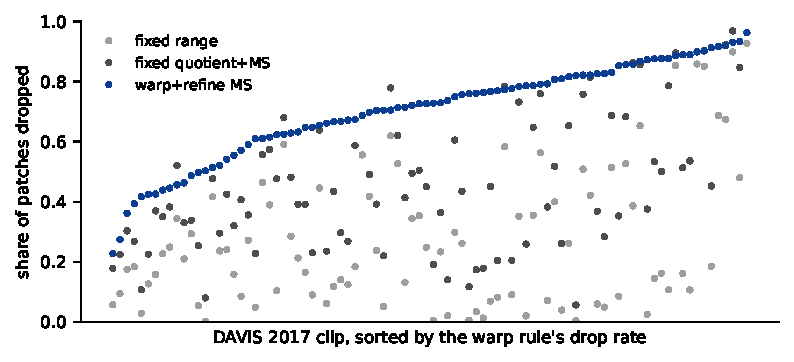
\includegraphics[width=0.66\linewidth]{figures/davis_drop}\hfill
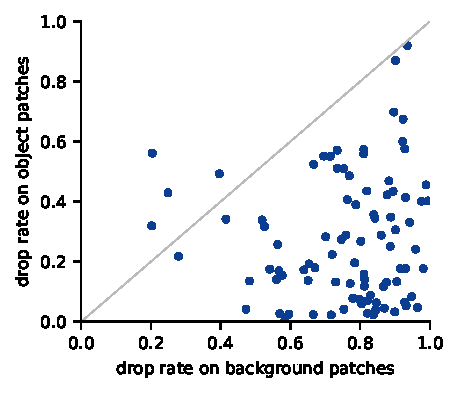
\includegraphics[width=0.33\linewidth]{figures/davis_object_vs_background}
\caption{Left: share of patches dropped on each DAVIS clip, sorted by the full warp rule. Right: for the full warp rule, drop rate on object patches against background patches, one point per clip; points below the diagonal drop less on the objects than on the background.}
\label{fig:davis}
\end{figure}

The full warp rule drops a median of 72.8\% of patches, against 43.5\% for the fixed-camera quotient + multi-scale rule and 21.2\% for the fixed range rule. It drops more than the fixed rule on 81 of the 90 clips, by a median of 20 points; across clips its drop rate runs from 46\% at the 10th percentile to 89\% at the 90th. Registration alone (warp range, 43.6\%) only matches the fixed quotient rule; the per-patch refinement adds six points and the multi-scale certificate another 23, which is the same order of gains as on fixed cameras: jitter of sharp edges, now including the residual jitter left by an imperfect homography, is what the range statistic spends its budget on.

The drop comes from the background. The full rule drops 80.7\% of background patches and 23.3\% of object patches, and it drops fewer object than background patches on 86 of the 90 clips. The objects in DAVIS move independently of the camera, so they are not explained by the frame warp and are mostly kept, which is the desired behaviour; what is dropped on objects is largely their interior, which can be locally static. About 4\% of patches are kept because their area has just entered the frame and has no reference, and registration fails on 22 of the 90 clips at least once (0.74 frames per clip on average), each time costing a full frame.

Soundness was re-checked with exact persistence diagrams on 20{,}242 dropped patches across the three warp rules (6{,}830 for the full rule), against the warped reference each rule constructed. There is no violation. The worst ratio of bottleneck distance to $s/2$ is 1.000 up to rounding: Theorem~\ref{thm:warp}(b) is attained and never exceeded, as on fixed cameras.

The price is the interpolation term. Its median over clips is 44 grey levels for the full rule. Per pixel, 4\% of the pixels of dropped patches have $\iota \le 0.5$, 69\% have $\iota \le 16$ and 96\% have $\iota \le 64$. So relative to the warped reference the certificate is exact at contrast $\Delta$, but relative to the kept pixels themselves it is, on a typical pixel, a statement at contrast $\Delta + 2\iota$, and on sharp edges a weak one. Section~\ref{sec:limits} returns to this.

\subsection{A film with cuts}

Tears of Steel (CC-BY, 720p) is cut like a feature film: handheld and dolly shots, close-ups, and a cut every few seconds. We take three 60-s excerpts starting at 120, 360 and 540~s, sampled at 6~fps and scaled to $960{\times}400$ (Table~\ref{tab:film}). The full warp rule drops 75\%, 75\% and 64\% of patches, against 65\%, 65\% and 54\% for the fixed-camera quotient + multi-scale rule. It treats 54 frames as cuts across the three excerpts, real shot changes and registration failures alike, and keeps every patch on each of them, so cut-heavy footage pays for its cuts. The certificate was re-checked on 2{,}046 dropped patches with no violation.

\begin{table}[t]
\centering\small
\begin{tabular}{lrrrrr}
\toprule
rule & drop, 120s & drop, 360s & drop, 540s & cuts & $\iota$ median \\
\midrule
fixed range & 0.478 & 0.496 & 0.310 & 0 & 0 \\
fixed quotient+MS & 0.650 & 0.653 & 0.543 & 0 & 0 \\
warp range & 0.635 & 0.630 & 0.421 & 54 & 21 \\
warp+refine range & 0.677 & 0.675 & 0.481 & 54 & 22 \\
warp+refine MS & 0.752 & 0.753 & 0.640 & 54 & 25 \\
\bottomrule
\end{tabular}

\caption{Tears of Steel, three 60-s excerpts at 6~fps. ``Cuts'' counts frames on which registration failed and the canvas was reset, summed over the excerpts; the fixed-camera rules have no notion of a cut.}
\label{tab:film}
\end{table}

\subsection{Soundness of the warp certificate on synthetic scenes}
\label{sec:warpaudit}

Footage cannot test the part of the argument that Proposition~\ref{prop:iota} leaves to measurement: whether the features of the kept content survive in the warped reference. Synthetic scenes can, because the content is known. Four scene types (smooth blobs, sharp edges, fine texture, and a mixture) are re-rendered under three warp families: whole-pixel translations, sub-pixel translations and random homographies (Table~\ref{tab:warpaudit}). Over 2{,}431 dropped patches there is no violation of Theorem~\ref{thm:warp} and none of Proposition~\ref{prop:iota}, either per pixel or on the diagrams, and in every configuration $W$ has at least as many features of contrast $\ge \Delta - 2\iota$ as the re-indexed kept pixels have of contrast $\ge \Delta$, 4{,}900 features in all. This is a count, not a matching: it shows that no $\Delta$-feature is lost to interpolation in number, not that each is matched to itself. Under whole-pixel translations $\iota$ is zero on every pixel, as the proposition says. Under sub-pixel warps its median is 8--24 grey levels, and it is largest on the edge and mixed scenes, which are also the scenes where the rule keeps most: of the 225 sub-pixel edge patches it drops 156, of the 204 homography edge patches 110.

\begin{table}[t]
\centering\scriptsize
\setlength{\tabcolsep}{4pt}
\begin{tabular}{llrrrrrr}
\toprule
warp & scene & dropped & Thm.~\ref{thm:warp} viol. & Prop.~\ref{prop:iota} viol. & $\iota$ median & $\iota$ p90 & $\Delta$-features surviving \\
\midrule
integer & smooth & 237/237 & 0 & 0 & 0.0 & 0.0 & 1.00 of 443 \\
integer & edges & 240/240 & 0 & 0 & 0.0 & 0.0 & 1.00 of 478 \\
integer & texture & 243/243 & 0 & 0 & 0.0 & 0.0 & 1.00 of 513 \\
integer & mixed & 253/253 & 0 & 0 & 0.0 & 0.0 & 1.00 of 569 \\
subpixel & smooth & 225/225 & 0 & 0 & 8.2 & 16.2 & 1.00 of 408 \\
subpixel & edges & 156/225 & 0 & 0 & 12.5 & 51.6 & 1.00 of 303 \\
subpixel & texture & 225/225 & 0 & 0 & 16.2 & 27.1 & 1.00 of 455 \\
subpixel & mixed & 163/225 & 0 & 0 & 24.0 & 75.5 & 1.00 of 345 \\
homography & smooth & 226/226 & 0 & 0 & 7.9 & 15.5 & 1.00 of 433 \\
homography & edges & 110/204 & 0 & 0 & 11.1 & 33.2 & 1.00 of 204 \\
homography & texture & 218/218 & 0 & 0 & 18.2 & 29.3 & 1.00 of 463 \\
homography & mixed & 135/222 & 0 & 0 & 20.2 & 74.3 & 1.00 of 286 \\
\bottomrule
\end{tabular}

\caption{Synthetic audit of the warp certificate. ``Viol.'' counts dropped patches on which the stated bound fails, checked with exact persistence diagrams. The last column counts features of contrast $\ge \Delta$ in the re-indexed kept pixels and the share of that count matched by features of $W$ of contrast $\ge \Delta - 2\iota$.}
\label{tab:warpaudit}
\end{table}

\subsection{The causal rule against the clairvoyant optimum}
\label{sec:compexp}

For every patch of three fixed-camera clips (hall monitor, the CAVIAR lobby, VIRAT) we compute the anchored rule's keeps $m_\theta$ and, by dynamic programming with full knowledge of the sequence, the fewest keeps $\OPT_\theta$ and $\OPT_{\theta/2}$ of any sound schedule, for the range statistic at $\theta \in \{16, 32, 48\}$ and the $L^1$ mean at $\theta \in \{2, 4, 8\}$ (Table~\ref{tab:competitive}). Theorem~\ref{thm:opt}(i) and (ii) hold on every patch. Summed over a clip, the ratio $m_\theta / \OPT_\theta$ is between 1.002 and 1.183 in all 18 settings: at the \emph{same} guarantee, the causal rule keeps at most 18\% more than a schedule that knows the future. The worst single patch is 16 times the optimum (lobby, range at 32), which is the unbounded gap of Section~\ref{sec:opt} occurring in practice on a handful of patches whose content alternates around a value the rule never anchors on. The factor two of Theorem~\ref{thm:opt}(ii) is far from binding: $\OPT_{\theta/2}$ is often several times $m_\theta$, because halving the guarantee costs any schedule more than causality costs the anchored rule.

\begin{table}[t]
\centering\scriptsize
\begin{tabular}{llrrrrrr}
\toprule
clip & statistic, $\theta$ & rule keeps $m_\theta$ & $\OPT_\theta$ & $\OPT_{\theta/2}$ & $m_\theta/\OPT_\theta$ & worst patch & viol. \\
\midrule
hall & range, 16 & 87809 & 83195 & 117900 & 1.055 & 6.0 & 0 \\
hall & range, 32 & 32391 & 30390 & 83195 & 1.066 & 8.2 & 0 \\
hall & range, 48 & 15997 & 13646 & 44358 & 1.172 & 7.0 & 0 \\
hall & mean, 2 & 99473 & 97869 & 114462 & 1.016 & 7.7 & 0 \\
hall & mean, 4 & 15776 & 14113 & 97869 & 1.118 & 8.7 & 0 \\
hall & mean, 8 & 5949 & 5829 & 14113 & 1.021 & 1.6 & 0 \\
lobby & range, 16 & 84108 & 83527 & 115852 & 1.007 & 3.0 & 0 \\
lobby & range, 32 & 31363 & 27685 & 83527 & 1.133 & 16.0 & 0 \\
lobby & range, 48 & 14917 & 12608 & 50386 & 1.183 & 13.0 & 0 \\
lobby & mean, 2 & 71807 & 71103 & 106241 & 1.010 & 3.8 & 0 \\
lobby & mean, 4 & 21347 & 18543 & 71103 & 1.151 & 12.3 & 0 \\
lobby & mean, 8 & 4638 & 3974 & 18543 & 1.167 & 8.5 & 0 \\
virat & range, 16 & 8719 & 7763 & 127710 & 1.123 & 11.0 & 0 \\
virat & range, 32 & 4545 & 4373 & 7763 & 1.039 & 3.0 & 0 \\
virat & range, 48 & 3939 & 3887 & 5149 & 1.013 & 3.0 & 0 \\
virat & mean, 2 & 5013 & 4841 & 67484 & 1.036 & 3.0 & 0 \\
virat & mean, 4 & 3670 & 3651 & 4841 & 1.005 & 3.0 & 0 \\
virat & mean, 8 & 3114 & 3107 & 3651 & 1.002 & 2.5 & 0 \\
\bottomrule
\end{tabular}

\caption{Keeps of the anchored rule against the clairvoyant optimum, summed over all patches of a clip. ``Worst patch'' is the largest per-patch ratio $m_\theta/\OPT_\theta$; ``viol.'' counts patches violating Theorem~\ref{thm:opt}(i) or (ii).}
\label{tab:competitive}
\end{table}

\subsection{The cost of refusing the brightness shift}
\label{sec:shiftexp}

Section~\ref{sec:shift} replaces the shift $c$, which a cached token cannot apply, by a keep rule: send the patch whenever $|c| > \kappa$. Table~\ref{tab:shift} and Figure~\ref{fig:shift} give the drop rate as a function of $\kappa$ on the three fixed-camera clips. At $\kappa = 16$ the keep rule costs 0.7, 0.6 and 0.3 points of drop rate for quotient + multi-scale (hall 94.9\% to 94.2\%, lobby 97.1\% to 96.5\%, VIRAT 99.4\% to 99.1\%) and at most 0.02 points for the range rule; the 99th percentile of $|c|$ over dropped patches is 10--15 grey levels. A tight cap is expensive: at $\kappa = 4$ the multi-scale rule falls to 80--92\%, and at $\kappa = 0$ almost nothing is dropped, because camera gain and compression move the brightness of a static patch by a few levels all the time. So a reused token can be held to $\Delta/2 + 16$ pointwise with nothing to apply, at under one point of drop rate; holding it to $\Delta/2$ exactly needs the shift to be applied inside the model.

\begin{table}[t]
\centering\scriptsize
\setlength{\tabcolsep}{3.5pt}
\begin{tabular}{llrrrrrrrrrr}
\toprule
clip & rule & $\kappa=0$ & $\kappa=1$ & $\kappa=2$ & $\kappa=4$ & $\kappa=8$ & $\kappa=16$ & $\kappa=32$ & $\kappa=\infty$ & $|c|$ p90 & $|c|$ p99 \\
\midrule
hall & range d=32 & 0.067 & 0.306 & 0.504 & 0.666 & 0.715 & 0.730 & 0.730 & 0.730 & 4 & 10 \\
hall & quotient+MS d0=80 & 0.005 & 0.300 & 0.560 & 0.804 & 0.900 & 0.942 & 0.949 & 0.949 & 5 & 15 \\
lobby & range d=32 & 0.121 & 0.444 & 0.622 & 0.731 & 0.761 & 0.763 & 0.763 & 0.763 & 3 & 6 \\
lobby & quotient+MS d0=80 & 0.015 & 0.337 & 0.574 & 0.802 & 0.928 & 0.965 & 0.971 & 0.971 & 5 & 14 \\
virat & range d=32 & 0.182 & 0.683 & 0.860 & 0.921 & 0.968 & 0.991 & 0.991 & 0.991 & 3 & 10 \\
virat & quotient+MS d0=80 & 0.001 & 0.596 & 0.837 & 0.915 & 0.953 & 0.991 & 0.994 & 0.994 & 3 & 12 \\
\bottomrule
\end{tabular}

\caption{Drop rate with the keep rule $|c| \le \kappa$, on three fixed-camera clips. $\kappa = \infty$ is the rule without the cap. The last two columns are percentiles of $|c|$ over dropped patches, in grey levels.}
\label{tab:shift}
\end{table}

\begin{figure}[t]
\centering
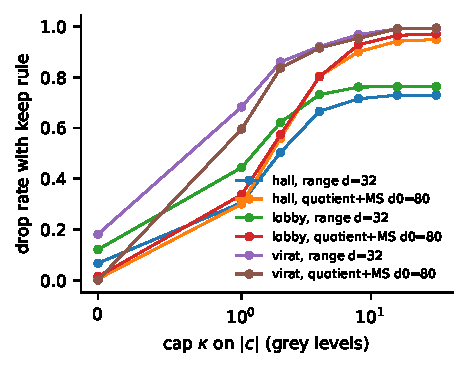
\includegraphics[width=0.55\linewidth]{figures/shift_cost}
\caption{Drop rate against the cap $\kappa$ on the brightness shift (Table~\ref{tab:shift}). Above $\kappa \approx 16$ the cap costs almost nothing.}
\label{fig:shift}
\end{figure}

\section{Limitations and open problems}
\label{sec:limits}

\paragraph{No token is reused inside a model.} Every result here is about which patches a rule sends, judged in pixels. Whether a video LLM fed only the sent patches answers as it does on full frames is measured in \citet{nair2026certifiedskip} on fixed cameras with a rebuilt-image protocol, and not at all on moving cameras. Doing it properly needs a model whose encoder accepts a sparse set of patches with their positions, plus the warp as metadata on frozen tokens. We have not built that.

\paragraph{No long-video benchmark.} There is no result on Video-MME \citep{fu2024videomme}, LongVideoBench \citep{wu2024longvideobench} or MLVU \citep{zhou2024mlvu}. Those benchmarks measure answer accuracy at a frame budget, and most of their footage is edited video at 1--2~fps, where a cut or a large change every few frames is the norm. The audit of Section~\ref{sec:audit} suggests what to expect there: at 2~fps the consecutive rules recover some slow change, and the advantage of anchoring shrinks to the events that a low rate makes look brief.

\paragraph{No certificate through a network.} The guarantee is on pixels. Section~\ref{sec:shift} explains why it does not pass through a standard encoder: dot-product attention is not Lipschitz on an unbounded domain, so the product of layer constants is undefined or vacuous. A certificate on tokens would need either an encoder built with bounded Lipschitz constants or a bound that uses the structure of real activations, and we claim neither.

\paragraph{The interpolation term is large on edges.} Theorem~\ref{thm:warp} is exact relative to the constructed reference $W$, but $W$ is a resampling of what was kept, and $\iota$ measures how far apart the two can be. On DAVIS its median over dropped patches is tens of grey levels, and on sharp edges it reaches the edge's contrast. Where $\iota$ is large, the statement relative to the kept pixels is weak, and Proposition~\ref{prop:iota} is honest about that rather than a fix for it. A reference built only from whole-pixel moves would make $\iota$ zero at the cost of keeping more under sub-pixel motion. The synthetic audit (Section~\ref{sec:warpaudit}) shows no loss of $\Delta$-features in number, which is weaker than a proof.

\paragraph{The competitive bound is for a fixed warp.} Theorem~\ref{thm:opt} holds for any seminorm on a fixed camera, and for the warp rule with the warp held fixed. When the warp changes between frames, the triangle inequality picks up an interpolation term and we state no bound. The measured ratios of Section~\ref{sec:compexp} are on fixed cameras only.

\paragraph{Speed.} The warp rule is a Python prototype and took about 1.0--1.4~s per 480p frame for registration, refinement and the canvas (nine clips in parallel on one laptop), against about 0.15~s for the fixed-camera rule in Python under the same load and hundreds of frames per second for its C++ core. Homography registration is cheap in principle and runs in real time in every video codec; the gap is engineering, not mathematics, but it has not been closed.

\paragraph{The audit tests decision rules, not systems.} Each reducer is reduced to its temporal comparison in pixel space (Appendix~\ref{app:reducers}). A learned feature can be more or less sensitive than the pixel statistic that replaces it, so the recall numbers are not those of the published systems. What carries over is the structural point: no feature, learned or not, sees a change against a frame it is not compared with. DyCoke's window of four frames was implemented but not run in this audit, PruneVid's clustering into segments and LongVU's query-guided and spatial steps are not re-implemented, and the attention-based reducers (FastV, VisionZip, SparseVLM) need the model and are out of scope.

\paragraph{Footage.} Fixed-camera results use three clips (hall monitor, a CAVIAR lobby, one VIRAT scene) for the audit, the competitive analysis and the shift cost; moving-camera results use DAVIS~2017 at 40 frames per clip and three excerpts of one film. The planted events are synthetic objects composited into real footage. A deployment would want a larger and more varied set of cameras, and real events with ground truth.


\bibliographystyle{plainnat}
\bibliography{refs}

\appendix
\section{The warp rule on a fixed camera is the range rule}
\label{app:parity}

With the identity warp, no per-patch refinement and a canvas written only at whole pixel positions, every read in \eqref{eq:W} lands on a canvas pixel with weight one, and every canvas pixel holds the value of the frame that last kept it, unresampled. Then $W = R$, the last copy sent, on every patch, $\iota \equiv 0$, and the warp rule's statistic is the range rule's. The repository checks this bit for bit: on a synthetic fixed-camera sequence with noise and a planted change, the keep masks of the two implementations are identical, their scores agree to floating-point precision, and the maximum of $\iota$ is exactly zero (test \texttt{test\_fixed\_camera\_is\_the\_range\_rule\_bit\_for\_bit} in \texttt{tests/test\_paper.py}).

\section{What each reducer re-implementation keeps}
\label{app:reducers}

Each rule maps frames and a threshold to a keep mask over patches and frames, with frame~0 kept, so that one calibration routine can set every rule to the same budget. None of them is the published system: the model-side parts (ViT features, attention scores, merging inside the LLM) are replaced by the pixel-space statistic that plays the same role. What is kept is the comparison structure, that is, the frame against which a token is judged redundant.

\begin{center}\small
\begin{tabular}{p{0.24\linewidth}p{0.36\linewidth}p{0.3\linewidth}}
\toprule
rule & keep test & stands in for \\
\midrule
consecutive mean & mean $|F_t - F_{t-1}|$ over the patch $\ge \tau$ & EVS's pixel test; a per-frame analogue of RLT's \\
consecutive cosine & cosine similarity of mean-removed random projections of the patch in $F_t$ and $F_{t-1}$ $\le 1 - \tau$ & TimeChat-Online, FrameFusion, DyCoke's adjacent-frame test (on encoder or LLM features there) \\
segment static & patch kept on every frame of its 16-frame segment iff the mean pairwise cosine of its vectors over the segment is $< 1 - \tau$, else once & PruneVid's static tokens of a segment (fixed segments, not clustering) \\
window similarity & whole frame dropped iff its mean cosine to the other frames of its 8-frame window is $\ge 1 - \tau$ & LongVU's temporal reduction (on DINOv2 features there) \\
consecutive + refresh & consecutive mean, plus every patch every 60 frames & a periodic keyframe \\
uniform & every $k$-th frame in full & fixed-rate frame sampling \\
anchored mean & mean $|F_t - R|$ $\ge \tau$, $R$ the last kept copy & the anchored rule without a certificate \\
\bottomrule
\end{tabular}
\end{center}

The vectors of the cosine rule are a fixed $256 \times 64$ Gaussian projection of the mean-removed patch, an untrained proxy for a linear patch embedding that, like a ViT embedding under cosine similarity, ignores brightness and compares texture; a learned encoder may be more or less sensitive to a given change, but it compares the same two frames.

\section{Planted events}
\label{app:events}

Events are added to the integer frames of an untouched clip before any rule sees them, at random patch-aligned positions, with sign chosen against the local brightness so that the object always has the stated contrast. A one-frame event (small $5{\times}5$ at contrast 40, tiny $3{\times}3$ at 48) is caught if its patch is kept on that frame. A mover ($6{\times}6$, contrast 40, 2~px per frame for 12 frames) is caught on the share of its frames on which the patch under it is kept. A faint object ($6{\times}6$, contrast 12, persistent for 3~s) is caught if its patch is kept within 1~s of its onset. A fade ($8{\times}8$ over 3~s, or $12{\times}12$ over 12~s, linearly to contrast 48) is caught if its patch is kept at or before the frame where the fade reaches contrast 32; the object then keeps its final contrast, so a late keep is recorded as a delay. Thresholds are calibrated on the clip without events, so planted events do not change the budget a rule is held to.

\begin{table}[h]
\centering\scriptsize
\setlength{\tabcolsep}{3.5pt}
\resizebox{\linewidth}{!}{\begin{tabular}{lrrrrrrrrr}
\toprule
rule & drop & tokens/s & small 5$\times$5 & tiny 3$\times$3 & fade 3 s & fade 12 s & mover & faint 12 & $\rho$ median \\
\midrule
certified range & 0.965 & 31 & 0.17 & 0.30 & 0.10 & 0.10 & 0.11 & 0.07 & 0.000 \\
certified quotient+MS & 0.962 & 33 & 1.00 & 1.00 & 1.00 & 0.95 & 0.91 & 0.07 & 0.000 \\
certified +sequential & 0.961 & 34 & 1.00 & 1.00 & 1.00 & 0.95 & 0.91 & 1.00 & 0.012 \\
anchored mean (no certificate) & 0.970 & 26 & 0.17 & 0.07 & 1.00 & 1.00 & 0.13 & 0.07 & 0.000 \\
consecutive mean (EVS, RLT) & 0.970 & 26 & 0.07 & 0.10 & 0.00 & 0.00 & 0.11 & 0.07 & 0.000 \\
consecutive cosine (DyCoke, FrameFusion) & 0.970 & 26 & 0.43 & 0.37 & 0.10 & 0.00 & 0.24 & 0.13 & 0.000 \\
segment static (PruneVid) & \multicolumn{9}{l}{cannot reach the budget at this frame rate} \\
frame similarity (LongVU) & 0.974 & 23 & 0.07 & 0.00 & 0.10 & 0.20 & 0.02 & 0.00 & 0.023 \\
consecutive + refresh every 60 & 0.970 & 26 & 0.00 & 0.10 & 0.15 & 0.10 & 0.04 & 0.07 & 0.012 \\
uniform frames & 0.957 & 38 & 0.03 & 0.03 & 0.25 & 0.90 & 0.05 & 0.13 & 0.043 \\
\bottomrule
\end{tabular}
}

\vspace{4pt}
\resizebox{\linewidth}{!}{\begin{tabular}{lrrrrrrrrr}
\toprule
rule & drop & tokens/s & small 5$\times$5 & tiny 3$\times$3 & fade 3 s & fade 12 s & mover & faint 12 & $\rho$ median \\
\midrule
certified range & 0.991 & 15 & 0.13 & 0.17 & 0.00 & 0.05 & 0.00 & 0.00 & 0.000 \\
certified quotient+MS & 0.992 & 15 & 1.00 & 1.00 & 1.00 & 0.95 & 0.93 & 0.00 & 0.000 \\
certified +sequential & 0.991 & 16 & 1.00 & 1.00 & 1.00 & 0.95 & 0.93 & 1.00 & 0.000 \\
anchored mean (no certificate) & 0.990 & 18 & 1.00 & 0.47 & 1.00 & 1.00 & 0.88 & 0.27 & 0.000 \\
consecutive mean (EVS, RLT) & 0.990 & 18 & 1.00 & 0.90 & 1.00 & 0.15 & 0.99 & 0.93 & 0.000 \\
consecutive cosine (DyCoke, FrameFusion) & 0.990 & 18 & 0.60 & 0.40 & 0.15 & 0.05 & 0.47 & 0.13 & 0.000 \\
segment static (PruneVid) & \multicolumn{9}{l}{cannot reach the budget at this frame rate} \\
frame similarity (LongVU) & 0.993 & 13 & 0.00 & 0.03 & 0.00 & 0.05 & 0.02 & 0.07 & 0.020 \\
consecutive + refresh every 60 & 0.986 & 25 & 0.03 & 0.03 & 0.00 & 0.25 & 0.01 & 0.00 & 0.010 \\
uniform frames & 0.993 & 13 & 0.00 & 0.00 & 0.05 & 0.20 & 0.01 & 0.00 & 0.007 \\
\bottomrule
\end{tabular}
}
\caption{The audit of Table~\ref{tab:audit} at 2~fps: CAVIAR lobby (top) and VIRAT (bottom).}
\label{tab:audit2fps}
\end{table}

\begin{figure}[h]
\centering
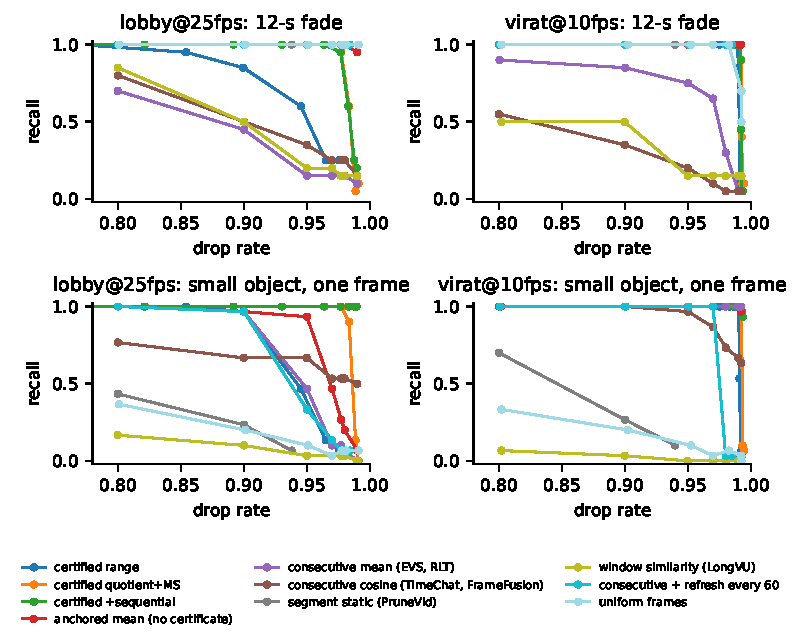
\includegraphics[width=\linewidth]{figures/audit_curves}
\caption{Recall of slow fades and of small objects against drop rate at the native frame rate, one panel per clip. Each curve is one rule swept over its threshold.}
\label{fig:auditcurves}
\end{figure}

\section{Computing the clairvoyant optimum}
\label{app:opt}

For one patch and a seminorm $\sigma$, $\OPT_\theta$ is the shortest sequence of keep times $0 = k_1 < k_2 < \dots$ such that every frame $t$ with anchor $k_j$ satisfies $\sigma(F_t - F_{k_j}) < \theta$. Let $\mathrm{reach}(k)$ be the last frame $t \ge k$ such that every frame in $[k, t]$ is within $\theta$ of $F_k$. A schedule is sound iff each keep's successor is at most $\mathrm{reach}(k) + 1$, so $\OPT_\theta$ is a shortest path on a DAG, computed by dynamic programming from the end of the sequence with $O(T^2)$ evaluations of $\sigma$ per patch. A brute-force search over all schedules confirms it on short random sequences. The anchored rule's keeps $m_\theta$ are counted on the same sequence, and Theorem~\ref{thm:opt}(i) and (ii) are checked on every patch (\texttt{scripts/competitive\_audit.py}).

\section{Reproducing the numbers}
\label{app:repro}

Every table and figure is generated from stored outputs by \texttt{scripts/make\_paper\_tables.py}. The outputs come from:

\begin{center}\scriptsize
\begin{tabular}{p{0.3\linewidth}p{0.62\linewidth}}
\toprule
result & command \\
\midrule
DAVIS (Table~\ref{tab:davis}) & \texttt{scripts/warp\_bench.py --davis all --frames 40} \\
film (Table~\ref{tab:film}) & \texttt{scripts/warp\_bench.py --film 120,360,540 --film-seconds 60} \\
synthetic audit (Table~\ref{tab:warpaudit}) & \texttt{scripts/warp\_audit.py} \\
competitive (Table~\ref{tab:competitive}) & \texttt{scripts/competitive\_audit.py --clips hall,lobby,virat --deltas 16,32,48} \\
shift cost (Table~\ref{tab:shift}) & \texttt{scripts/shift\_cost.py --clips hall,lobby,virat} \\
reducer audit (Tables~\ref{tab:audit}, \ref{tab:audit2fps}) & \texttt{scripts/audit\_reducers.py --clips lobby,virat --rates native,2} \\
\bottomrule
\end{tabular}
\end{center}

The theorems' finite claims are covered by \texttt{tests/test\_paper.py}: the fixed-camera parity of Appendix~\ref{app:parity}, registration of a synthetic pan, Theorem~\ref{thm:warp} against the constructed reference, the oscillation bound behind Proposition~\ref{prop:iota}, cut handling, Theorem~\ref{thm:opt}(i)--(ii) on random walks, optimality of the dynamic program by brute force, the adversary of Theorem~\ref{thm:opt}(iii), and Proposition~\ref{prop:consecutive} on a slow ramp for the re-implemented reducers. Footage is fetched by \texttt{scripts/fetch\_data.py}; DAVIS~2017 and Tears of Steel are under their own licences.


\end{document}
